\noindent
\begin{minipage}[t]{0.24\textwidth}
    \mbox{}
\end{minipage}%
\hfill
\begin{minipage}[t]{0.73\textwidth}
    Trong Ví dụ 6, chúng ta đã dùng quy tắc l'Hospital để chỉ ra rằng
    \begin{equation*}
        \lim_{x \to 0^+} x \ln x = 0
    \end{equation*}
    \vspace{-4pt}
    \noindent
    Do đó\hfill $\displaystyle \lim_{x \to 0^+} x^x = \lim_{x \to 0^+} e^{x \ln x} = e^0 = 1$ \hfill {\color{stewartcyan}\rule{1.2ex}{1.2ex}}
\end{minipage}

\vspace{10pt}

\noindent
\begin{tikzpicture}[x=1cm, y=1cm]
    \draw[stewartcyan, line width=1.5pt] (0, 0.45) -- (\linewidth, 0.45);
    \draw[stewartcyan, line width=0.5pt] (0, 0.35) -- (\linewidth, 0.35);
    
    \node[anchor=west, inner sep=0pt] at (0, 0) {
        {\color{stewartcyan}\fontsize{18}{22}\selectfont\bfseries\sffamily 4.4}
        \hspace{0.8em}
        {\color{black}\fontsize{18}{22}\selectfont\bfseries\sffamily Bài tập}
    };
    
    \draw[stewartcyan, line width=0.5pt] (3.8, 0.12) -- (\linewidth, 0.12);
    \draw[stewartcyan, line width=0.5pt] (3.8, 0.02) -- (\linewidth, 0.02);
    \draw[stewartcyan, line width=0.5pt] (3.8, -0.08) -- (\linewidth, -0.08);
    \draw[stewartcyan, line width=0.5pt] (3.8, -0.18) -- (\linewidth, -0.18);
    
    \draw[stewartcyan, line width=0.5pt] (0, -0.38) -- (\linewidth, -0.38);
    \draw[stewartcyan, line width=1.5pt] (0, -0.48) -- (\linewidth, -0.48);
\end{tikzpicture}

\vspace{8pt}

\noindent
\begin{minipage}[t]{0.485\textwidth}
    {\color{stewartcyan}\bfseries 1--4}\enskip Cho biết
    \begin{gather*}
        \lim_{x \to a} f(x) = 0 \qquad \lim_{x \to a} g(x) = 0 \qquad \lim_{x \to a} h(x) = 1 \\
        \lim_{x \to a} p(x) = \infty \qquad \lim_{x \to a} q(x) = \infty
    \end{gather*}
    giới hạn nào sau đây là dạng vô định? Đối với bất kỳ giới hạn nào không phải dạng vô định, hãy tính giá trị nếu có thể.

    \vspace{6pt}
    \noindent\textbf{1.}\enskip
    \begin{tabular}[t]{@{}p{0.46\linewidth}@{\hspace{0.04\linewidth}}p{0.46\linewidth}@{}}
        (a) $\lim\limits_{x \to a} \dfrac{f(x)}{g(x)}$ & (b) $\lim\limits_{x \to a} \dfrac{f(x)}{p(x)}$ \\[11pt]
        (c) $\lim\limits_{x \to a} \dfrac{h(x)}{p(x)}$ & (d) $\lim\limits_{x \to a} \dfrac{p(x)}{f(x)}$ \\[11pt]
        (e) $\lim\limits_{x \to a} \dfrac{p(x)}{q(x)}$ &
    \end{tabular}

    \vspace{5pt}
    \noindent\textbf{2.}\enskip
    \begin{tabular}[t]{@{}p{0.46\linewidth}@{\hspace{0.04\linewidth}}p{0.46\linewidth}@{}}
        (a) $\lim\limits_{x \to a} [f(x)p(x)]$ & (b) $\lim\limits_{x \to a} [h(x)p(x)]$ \\[9pt]
        (c) $\lim\limits_{x \to a} [p(x)q(x)]$ &
    \end{tabular}

    \vspace{5pt}
    \noindent\textbf{3.}\enskip
    \begin{tabular}[t]{@{}p{0.46\linewidth}@{\hspace{0.04\linewidth}}p{0.46\linewidth}@{}}
        (a) $\lim\limits_{x \to a} [f(x) - p(x)]$ & (b) $\lim\limits_{x \to a} [p(x) - q(x)]$ \\[9pt]
        (c) $\lim\limits_{x \to a} [p(x) + q(x)]$ &
    \end{tabular}

    \vspace{5pt}
    \noindent\textbf{4.}\enskip
    \begin{tabular}[t]{@{}p{0.46\linewidth}@{\hspace{0.04\linewidth}}p{0.46\linewidth}@{}}
        (a) $\lim\limits_{x \to a} [f(x)]^{g(x)}$ & (b) $\lim\limits_{x \to a} [f(x)]^{p(x)}$ \\[9pt]
        (c) $\lim\limits_{x \to a} [h(x)]^{p(x)}$ & (d) $\lim\limits_{x \to a} [p(x)]^{f(x)}$ \\[9pt]
        (e) $\lim\limits_{x \to a} [p(x)]^{q(x)}$ & (f) $\lim\limits_{x \to a} \sqrt[q(x)]{p(x)}$
    \end{tabular}

    \vspace{8pt}
    \noindent{\color{stewartcyan!60}\rule{\linewidth}{0.6pt}}
    \vspace{3pt}

    {\color{stewartcyan}\bfseries 5--6}\enskip Sử dụng đồ thị của $f$ và $g$ cùng các tiếp tuyến của chúng tại $(2, 0)$ để tìm $\lim\limits_{x \to 2} \dfrac{f(x)}{g(x)}$.

    \vspace{4pt}
    \begin{center}
        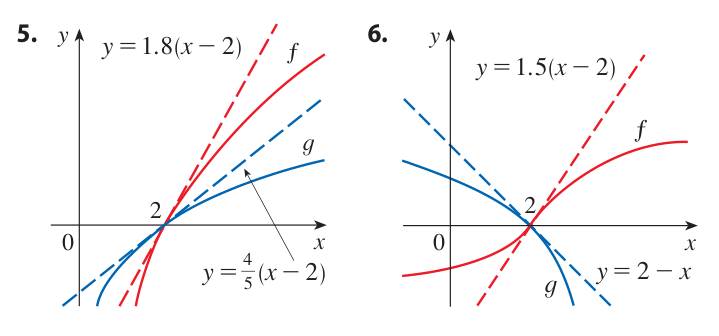
\includegraphics[width=\linewidth]{images/p0351_fig2.png}
    \end{center}
\end{minipage}%
\hfill
\begin{minipage}[t]{0.485\textwidth}
    \noindent\textbf{7.}\enskip Đồ thị của hàm số $f$ và tiếp tuyến của nó tại $0$ được cho như hình vẽ. Giá trị của $\lim\limits_{x \to 0} \dfrac{f(x)}{e^x - 1}$ bằng bao nhiêu?

    \vspace{2pt}
    \begin{center}
        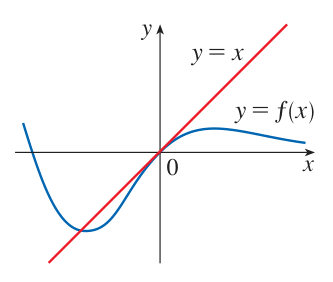
\includegraphics[width=0.60\linewidth]{images/p0351_fig1.png}
    \end{center}

    \vspace{2pt}
    \noindent
    {\color{stewartcyan}\bfseries 8--70}\enskip Tìm giới hạn. Hãy sử dụng quy tắc l’Hospital khi thích hợp. Nếu có phương pháp sơ cấp hơn, hãy cân nhắc sử dụng. Nếu quy tắc l’Hospital không áp dụng được, hãy giải thích lý do.

    \vspace{5pt}
    \noindent
    \begin{tabular}{@{}p{0.50\linewidth}@{\hspace{0.02\linewidth}}p{0.48\linewidth}@{}}
        \textbf{8.}\enskip $\lim\limits_{x \to 3} \dfrac{x - 3}{x^2 - 9}$ & \\[11pt]
        \textbf{9.}\enskip $\lim\limits_{x \to 4} \dfrac{x^2 - 2x - 8}{x - 4}$ & \textbf{10.}\enskip $\lim\limits_{x \to -2} \dfrac{x^3 + 8}{x + 2}$ \\[13pt]
        \textbf{11.}\enskip $\lim\limits_{x \to 1} \dfrac{x^7 - 1}{x^3 - 1}$ & \textbf{12.}\enskip $\lim\limits_{x \to 4} \dfrac{\sqrt{x} - 2}{x - 4}$ \\[13pt]
        \textbf{13.}\enskip $\lim\limits_{x \to \pi/4} \dfrac{\sin x - \cos x}{\tan x - 1}$ & \textbf{14.}\enskip $\lim\limits_{x \to 0} \dfrac{\tan 3x}{\sin 2x}$ \\[13pt]
        \textbf{15.}\enskip $\lim\limits_{t \to 0} \dfrac{e^{2t} - 1}{\sin t}$ & \textbf{16.}\enskip $\lim\limits_{x \to 0} \dfrac{x^2}{1 - \cos x}$ \\[13pt]
        \textbf{17.}\enskip $\lim\limits_{x \to 1} \dfrac{\sin(x - 1)}{x^3 + x - 2}$ & \textbf{18.}\enskip $\lim\limits_{\theta \to \pi} \dfrac{1 + \cos\theta}{1 - \cos\theta}$ \\[13pt]
        \textbf{19.}\enskip $\lim\limits_{x \to \infty} \dfrac{\sqrt{x}}{1 + e^x}$ & \textbf{20.}\enskip $\lim\limits_{x \to \infty} \dfrac{x + x^2}{1 - 2x^2}$ \\[13pt]
        \textbf{21.}\enskip $\lim\limits_{x \to 0^+} \dfrac{\ln x}{x}$ & \textbf{22.}\enskip $\lim\limits_{x \to \infty} \dfrac{\ln\sqrt{x}}{x^2}$ \\[13pt]
        \textbf{23.}\enskip $\lim\limits_{x \to 3} \dfrac{\ln(x/3)}{3 - x}$ & \textbf{24.}\enskip $\lim\limits_{t \to 0} \dfrac{8^t - 5^t}{t}$ \\[13pt]
        \textbf{25.}\enskip $\lim\limits_{x \to 0} \dfrac{\sqrt{1 + 2x} - \sqrt{1 - 4x}}{x}$ & \textbf{26.}\enskip $\lim\limits_{u \to \infty} \dfrac{e^{u/10}}{u^3}$ \\[13pt]
        \textbf{27.}\enskip $\lim\limits_{x \to 0} \dfrac{e^x + e^{-x} - 2}{e^x - x - 1}$ & \textbf{28.}\enskip $\lim\limits_{x \to 0} \dfrac{\sinh x - x}{x^3}$
    \end{tabular}
\end{minipage}

\vfill
\noindent{\color{stewartcyan!60}\rule{\textwidth}{0.5pt}}\\[3pt]
\parbox{\textwidth}{\fontsize{6.5pt}{8pt}\selectfont \color{black!70}
Copyright 2021 Cengage Learning. All Rights Reserved. May not be copied, scanned, or duplicated, in whole or in part. WCN 02-200-203\\
Editorial review has deemed that any suppressed content does not materially affect the overall learning experience. Cengage Learning reserves the right to remove additional content at any time if subsequent rights restrictions require it.}
